\section{Realizzazione DBMS}

Un \textbf{\textcolor{purple}{DBMS}} è un sistema software che
gestisce grandi quantità di dati, si và incontro
a problemi di efficienza, che sono \emph{\textcolor{purple}{persistenti}}, quindi il sistema
deve garantire affidabilità, e \emph{\textcolor{purple}{condivisi}}, in questo caso deve gestire il
controllo degli accessi e della concorrenza. La condivisione dei dati
è importante perchè permette di evitare la ridondanza dei dati (che porterebbe ad un spreco di memoria),
ma può anche portare a problemi di inconsistenza, dato che se si hanno tante copie
di un dato, una modifica di una sola delle copie deve essere propagata nelle altre.

A causa della sua dimensione, un database risiede normalmente
sui dischi, e prima che i suoi dati debbano essere elaborati dal
DBMS, questi devono essere trasferiti in memoria centrale. Questo
trasferimento non coinvolge le singolo tuple ma è effettuato
a \textcolor{purple}{blocchi} o \textcolor{purple}{pagine}.

Un \textcolor{purple}{blocco}, fisicamente, è una sequenza
continua di settori di una traccia, costituendo l'unità di trasferimento
dati da e per la memoria principale. La dimensione tipica è tra i 4 - 64 KB.

\paragraph{\textcolor{purple}{Struttura della Pagina}} Una pagina, logicamente,
è formata da alcune informazioni di servizio e da un'area dove sono contenuti
dei \emph{record}. Il riferimento ad un record, chiamato \textbf{RID} è formato
dalla coppia (\textbf{PID} della pagina, posizione del record nella pagina).

\begin{figure}[H]
    \centering
    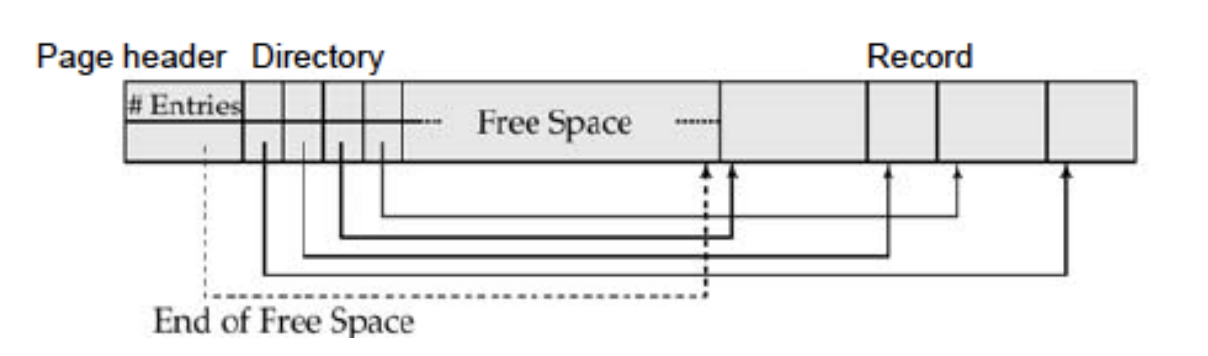
\includegraphics[scale=0.55]{img/rid.png}
\end{figure}

La \textcolor{purple}{directory} contiene un puntatore per ogni record
della pagina, in questo modo è possibile riallocare il record nella pagina
senza modificare il \textbf{RID}.

\subsection{Gestore Memoria}

L'architettura a livello fisico è la seguente.
\begin{figure}[H]
    \centering
    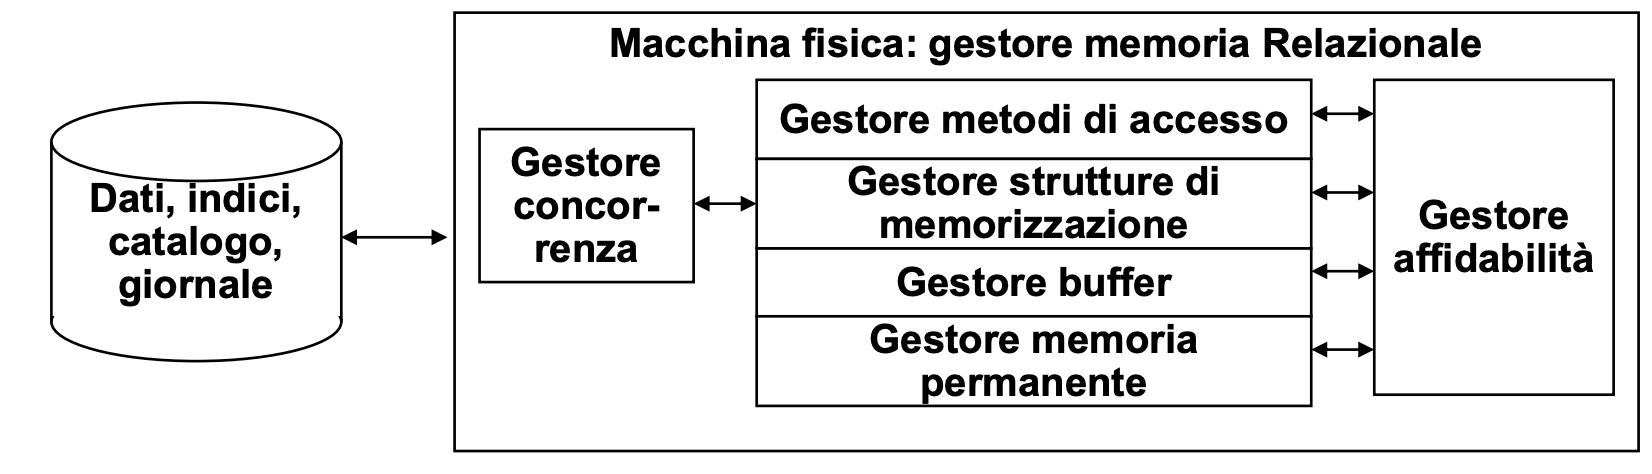
\includegraphics[scale=0.4]{img/macchina_fisica.png}
\end{figure}

\begin{itemize}
    \item \textcolor{purple}{Gestore Memoria Permanente}: fornisce un'astrazione della memoria
        permanente sotto forma di insiemi di file logici di blocchi fisici, nascondendo
        le caratteristiche dei dischi e dell'OS.
    \item \textcolor{purple}{Gestore del Buffer}: si occupa del trasferimento delle pagine
        tra la memoria temporanea e quella permanente, offrendo ai livelli superiore
        una visione della memoria permanente come un insieme di pagine utilizzabili in quella temporanea.
        In questo modo viene nascosta l'operazione di trasferimento.
            \begin{figure}[H]
                \centering
                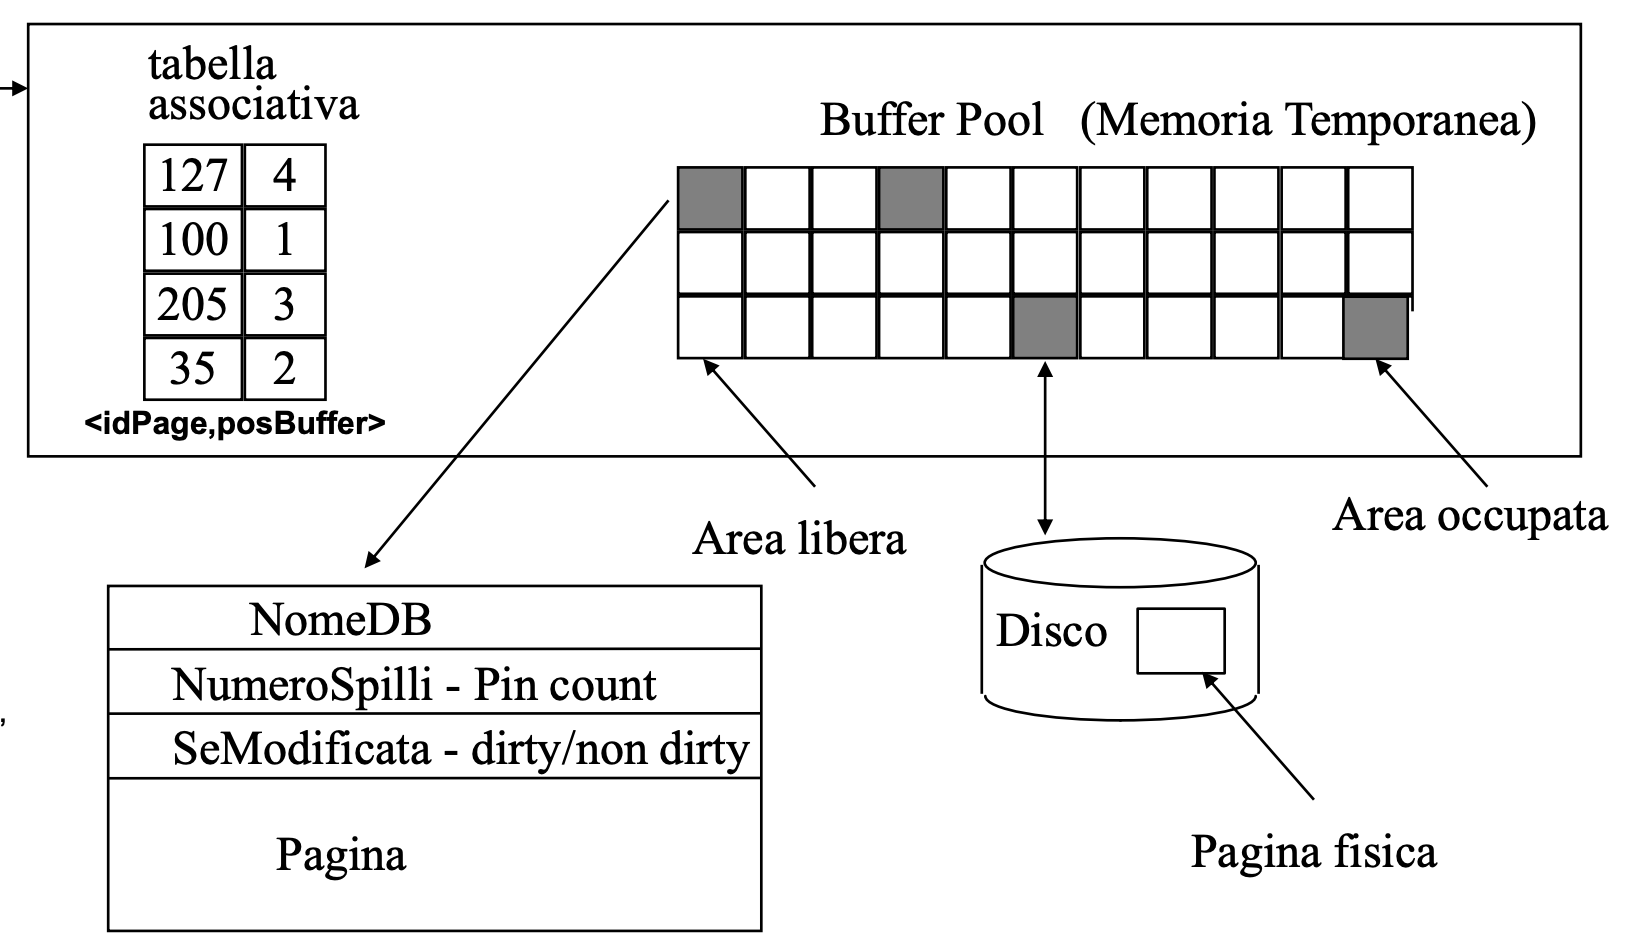
\includegraphics[scale=0.4]{img/buffer.png}
            \end{figure}
        Nell'header della pagina presente nella memoria temporanea, \emph{Pin Count}
        viene incrementato se la pagina viene richiesta e decrementato se viene rilasciata.
        Vengono utilizzate alcune primitive:
        \begin{itemize}
            \item \verb|getAndPinPage(x)|: indica la richiesta al buffer della pagina
                con \verb|idPage = x| e viene incrementato il \verb|pin count| relativo a quella
                pagina per indicarne l'uso.
            \item \verb|unPinPage(x)|: rilascia una pagina e decrementa il \emph{pin count}.
            \item \verb|setDirty(x)|: imposta il bit \verb|dirty| a 1, che indica se la pagina
                è stata modificata.
            \item \verb|flushPage(x)|: forza la scrittura della pagina su disco ed imposta il bit \verb|dirty|
                a 0.
        \end{itemize}
    \item \textcolor{purple}{Gestore Strutture di Memorizzazione}: ogni tipo di organizzazione ha i suoi
        pro e contro, basandoci sul costo delle operazioni che effettuiamo sui dati e sulla sua occupazione
        in memoria.
        \begin{itemize}
            \item \textcolor{purple}{Organizzazione Seriale} o \textcolor{purple}{Heap File}: i dati sono memorizzati
                in modo casuale uno dopo l'altro, il costo in memoria è basso ma è poco efficiente per le operazioni.
            \item \textcolor{purple}{Organizzazione Sequenziale}: i dati vengono ordinati sul valore di uno o più attributi,
                le inserizioni fanno perdere l'ordinamento, ma le ricerche sono più veloci, dato che si applica la ricerca
                binaria. Se un file contiene un numero di pagine uguale a \verb|b| allora occorreranno un numero di accessi
                uguale a $\log_{2}{b}$ per individuare il record.
            \item \textcolor{purple}{Organizzazioni Per Chiave}: in queste organizzazioni, noto il valore di una
                chiave si trova il record di una tabella con un numero di accessi al disco che dovrebbe essere
                idealmente uguale ad 1.
        \end{itemize}
\end{itemize}

\subsection{Organizzazioni Per Chiave}

\subsubsection{Hash File}
In un file hash, i record vengono allocati in una pagina il cui indirizzo dipende dal
valore di chiave del record stesso. Ad esempio, se un record ha chiave $k$ allora si inserisce
nella pagina di indirizzo $H(k)$, dove $H(k) = k \mod NrPage$.

Le collisioni sono gestite con delle \emph{Linked List}. Questa organizzazione è la più
efficiente se si considera solo l'accesso diretto basato sui valori della chiave con condizioni
di uguaglianza. Non è efficiente invece per ricerche basate su intervalli o su attributi diversi dalla
chiave. Inoltre è un'organizzazione \textcolor{purple}{procedurale statica}, quindi funziona solo
su file la cui dimensione varia poco nel tempo.

Invece, gli svantaggi che riguardano puramente la struttura dipendono dal numero di pagine, se è troppo
piccolo rispetto alla dimensione del database si hanno frequenti collisioni, altrimenti se è troppo grande il
fattore di riempimento delle pagine è molto basso.

\subsubsection{Metodo Tabellare}

Si usa un \textcolor{purple}{indice}, ovvero un insieme ordinato
di coppie \verb|(k, r(k))|, dove \verb|k| è un valore della chiave ed \verb|r(k)|
è un riferimento al record con chiave \verb|k|. Gli indici possono essere
su più attributi. L'indice viene gestito con una struttura chiamata
$B^+-tree$. Prima di vedere i $B^+-tree$, vediamo i $B-tree$, dove fissato l'ordine
$p$, questi rappresentano degli alberi di ricerca dove ogni nodo interno ha questa forma:
\begin{equation*}
    <P_1, <K_1, Pr_1>, P_2, <K_2, Pr_2>, \dots, <K_{q-1}, Pr_{q-1}>, P_q>
\end{equation*}
dove $q \leq p$. I $P_i$ sono chiamati \emph{tree pointer} ovvero rappresentano
un puntatore ad un altro node del $B-tree$, $K_i$ è la chiave di ricerca, e $Pr_i$
è un \emph{data pointer}, ovvero è un puntatore ad un record il cui campo \emph{chiave di ricerca}
è uguale a $K_i$ oppure ad una pagine che contiene tale record.
Per ogni nodo vale la proprietà $K_1 < K_2 < \dots < K_{q-1}$, e deve avere al massimo
$p$ \emph{tree pointer}.

\begin{figure}[H]
    \centering
    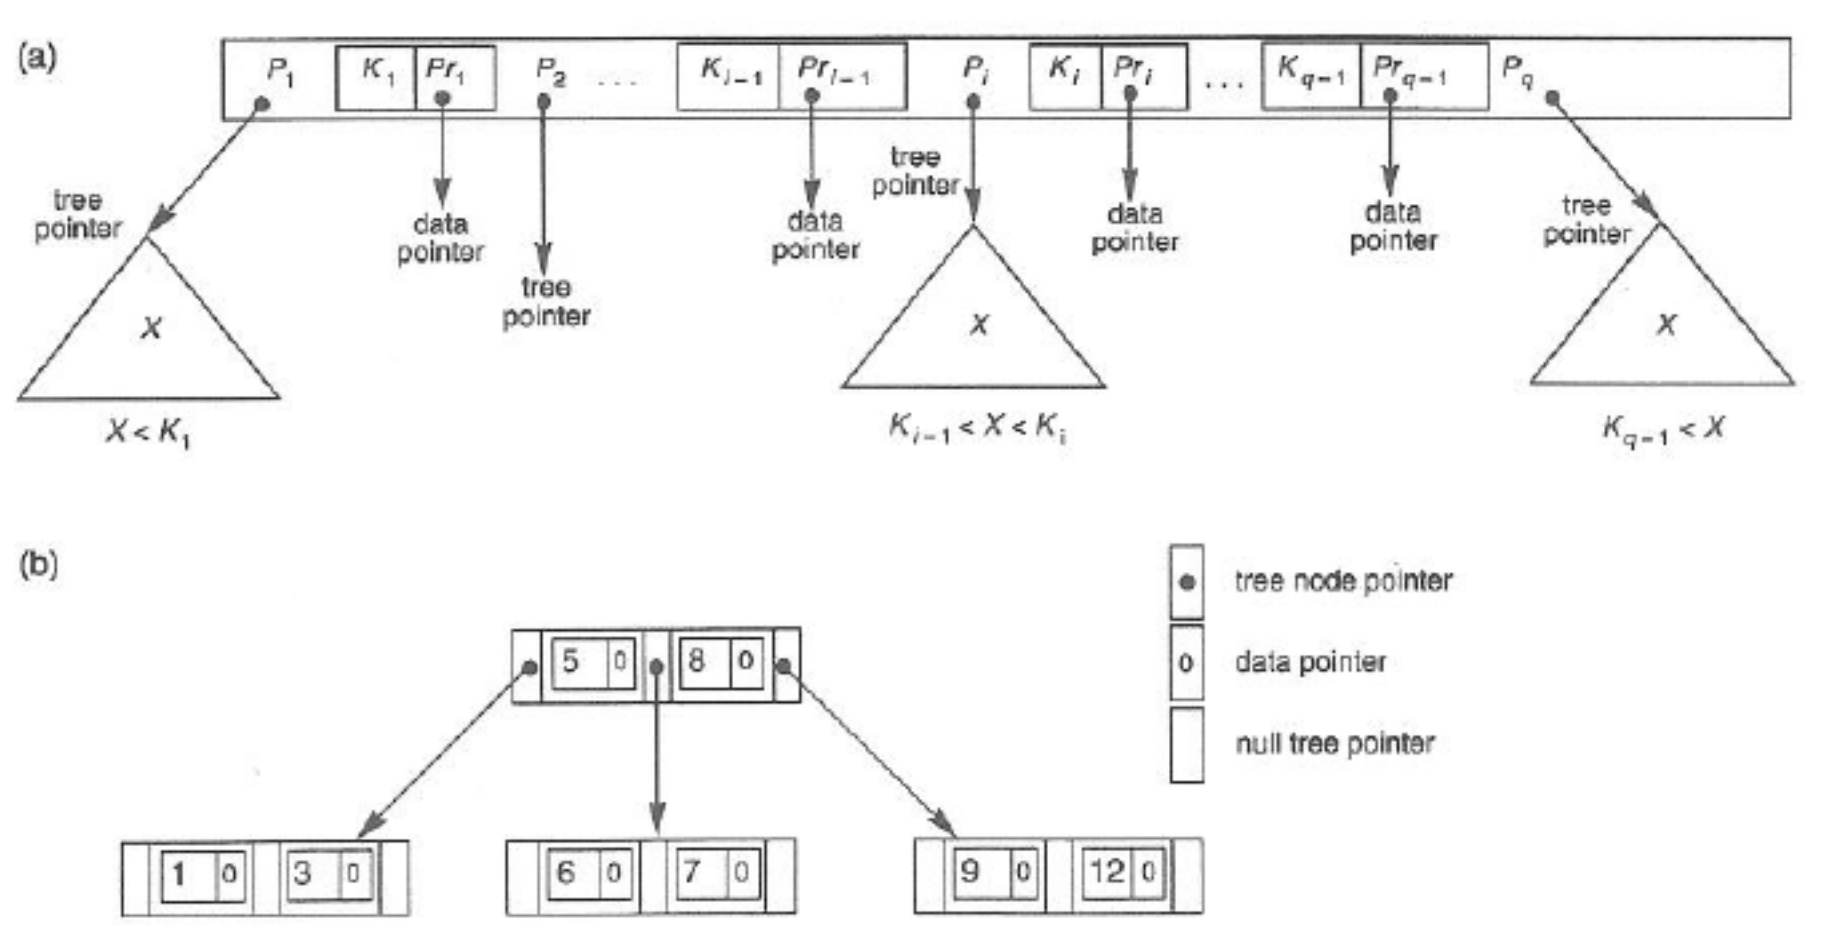
\includegraphics[scale=0.37]{img/btree.png}
\end{figure}

Per tutti i valori $X$ della chiave di ricerca che appartengono al
sottoalbero puntato da $P_i$ vale che:
\begin{equation*}
    K_{i-1} < X < K_i \;\;per\; 1 < i < q
\end{equation*}
\begin{equation*}
    X < K_i \;\;per\; i = 1
\end{equation*}
\begin{equation*}
    K_{i-1} < X \;\;per\; i = q
\end{equation*}

I vincoli che il $B-tree$ deve rispettare, che lo differenziano da un normale
albero di ricerca sono:
\begin{itemize}
    \item La radice ha almeno due \emph{tree pointer} a meno che non sia l'unico nodo.
    \item Ogni nodo, esclusa la radice, ha almeno $\lceil \frac{p}{2} \rceil$
        \emph{tree pointer}.
    \item Tutti i nodi foglia sono posti sullo stesso livello.
\end{itemize}
Questi vincoli garantiscono che il $B-tree$ sia bilanciato. \\

I $B^+-tree$, sono essenzialmente dei $B-tree$ dove i \emph{data pointer} sono memorizzati
esclusivamente nei nodi foglia dell'albero. Quindi, fissato l'ordine $p$, ogni nodo interno
ha la seguente forma:
\begin{equation*}
    <P_1, K_1, P_2, K_2, \dots, P_{q-1}, K_{q-1}, P_q>
\end{equation*}
con $q \leq p$.
Un'altra piccola differenza è che per ogni valore $X$ della chiave di ricerca
puntata da $P_i$ si ha che:
\begin{equation*}
    X \leq K_i \;\;per\; i = 1
\end{equation*}
\begin{equation*}
    K_{i-1} < X \leq K_i \;\;per\; 1 < i < q
\end{equation*}
\begin{equation*}
    K_{i-1} < X \;\;per\; i = q
\end{equation*}

\begin{figure}[H]
    \centering
    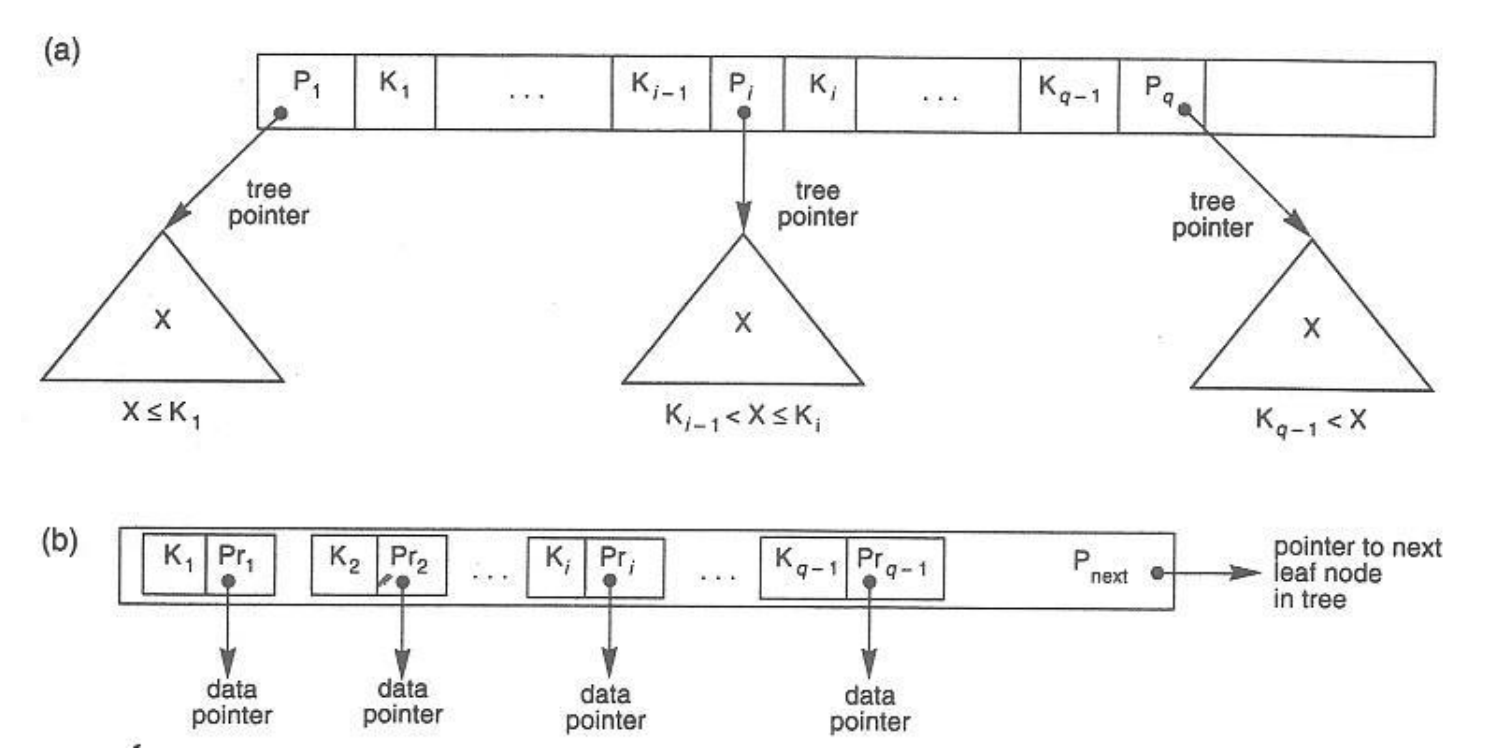
\includegraphics[scale=0.46]{img/b+tree.png}
\end{figure}

La struttura dei nodi foglia è la seguente:
\begin{equation*}
    <<K_1, Pr_1>, <K_2, Pr_2>, \dots, <K_q, Pr_q> P_{next}>
\end{equation*}
dove $q \leq p_{leaf}$ e dove vale sempre $K_1 < K_2 < \dots < K_q$.
$P_{next}$ è un \emph{tree pointer} che punta al successivo nodo foglia
del $B^+-tree$. Ogni $Pr_i$, invece, è un \emph{data pointer} che punta al record
con campo di ricerca uguale a $K_i$, a un blocco contenente tale record, o a un blocco
di puntatori ai record con campo di ricerca uguale a $K_i$, se il campo di ricerca non è una
chiave. Ogni nodo foglia ha almeno $\lceil \frac{p_{leaf}}{2} \rceil$ valori. 

Ovviamente è importante sottolineare che gli alberi stessi sono memorizzati su disco,
assegnando ad ogni nodo una pagina. \\

Esistono due tipologie di indici ad albero:
\begin{itemize}
    \item \textcolor{purple}{Indici Statici}: la struttura ad albero viene creata sulla
        base dei dati presenti nel database e non viene più modificata se non periodicamente.
    \item \textcolor{purple}{Indici Dinamici}: la struttura ad albero viene aggiornata ad
        ogni operazione di inserimento e cancellazione.
\end{itemize}

Gli indici si possono anche distinguere in:
\begin{itemize}
    \item \textcolor{purple}{Indici Primari}: in questo caso la chiave di ordinamento del
        file sequenziale coincide con la chiave di ricerca dell'indice. È costituito da un insieme
        di coppie \verb|<K(i), RID(i)>|, dove il primo campo è la chiave primaria ed è dello stesso tipo
        del campo chiave di ordinamento, mentre il secondo campo è un puntatore ad un blocco del disco.
    \item \textcolor{purple}{Indici Secondari}: qui invece la chiave di ordinamento e quella
        di ricerca sono diverse. Questo indice può essere definito su un
        campo che non è chiave ma è chiave candidata, quindi ha valori univoci, oppure su un campo
        che ha valori duplicati. In questo caso il primo campo della coppia è chiamato campo di indicizzazione.
\end{itemize}

\subsection{Ordinamento}

L'ordinamento delle tabelle è importante non solo per ottenere
il risultato di un \verb|ORDER BY|, ma anche in altre operazioni relazionali
come la \verb|JOIN| e la \verb|GROUP BY| per ottimizzare i tempi.

L'algoritmo più usato dai \emph{DBMS} è il \textbf{\textcolor{purple}{Merge Sort a Z vie}},
dove a \emph{Z vie} indica che l'operazione di merge viene eseguita su \emph{Z} pagine alla volta.
Se si suppone di avere un file di $NP$ pagine e di avere un numero di
buffer $NB < NP$ in memoria centrale; l'algoritmo opera in due step:
\begin{itemize}
    \item Prima esegue un sort interno, utilizzando ad esempio il \emph{Quicksort}, in cui all'interno di ogni pagina
        i record vengono ordinati, le pagine ordinate vengono chiamate \emph{\textcolor{purple}{run}}.
    \item Infine, operando uno o più passi di fusione, in base al numero di vie usate, le \emph{run} vengono fuse fino a produrne una sola.
\end{itemize}

Supponendo di avere a diposizione $NB = 3$ buffer, dove due sono quelli
di input e uno è quello di output, e di considerare nel calcolo della complessità
solo il numero di operazioni \emph{I/O} effettuate tra memoria centrale e fisica.

Nella fase di sort interno, si scriverà ogni pagina in uno dei buffer di input
e poi si riscriverà ordinata in quello di output, impiegando un numero di operazioni uguale
a $2 \cdot NP$. Ad ogni passo di merge in totale si leggeranno e scriveranno
sempre $2 \cdot NP$ pagine (i record bisogna visitarli sempre tutti), e il numero di passi di merge sarà $\lceil \log_{2}NP \rceil$ in quanto
ad ogni passo il numero di \emph{run} si dimezza. Il costo totale è quindi
pari a $2 \cdot NP \cdot (\lceil \log_{2}NP \rceil + 1)$.

Si può osservare che avendo a disposizione $NB$ buffer si possono ordinare $NP$ pagine
alla volta nella fase di sort interno anzichè una sola, il che porta ad un costo di $2 \cdot NP \cdot (\lceil \log_{2}{\frac{NP}{NB}} \rceil + 1)$.

Inoltre se abbiamo $NB > 3$ buffer si possono fondere $NB - 1$ run alla volta (1 buffer è per l'output).
In questo caso il costo è $2 \cdot NP \cdot (\lceil \log_{NB - 1}{\frac{NP}{NB}} \rceil + 1)$.

\subsubsection{JOIN}

Il costo di una \verb|JOIN| può essere molto elevato, dato che il prodotto
cartesiano tra due tabelle è molto grande, e questo seguito da una restrizione
può risultare inefficiente. Inoltre, anche se \verb|JOIN| è commutativo, la scelta
tra l'operatore da posizionare a sinistra e tra quello da posizionare a destra è cruciale
dal punto di vista dell'ottimizzazione computazionale.

Esistono 4 algoritmi per l'implementazione del \verb|JOIN|, chiameremo con $R$ la relazione a sinistra
(anche detta esterna), e con $S$ la relazione a destra (interna):
\begin{itemize}
    \item \textcolor{purple}{Nested Loops}: qui il costo dipende dallo spazio
        a disposizione in memoria centrale, nel caso si ha solo un buffer per $R$ e uno
        per $S$, bisogna caricare ogni pagina di $R$ e per ogni record della pagina
        si carica ogni volta una pagina di $S$, quindi il numero di operazioni di \emph{I/O}
        diventa $NPage(R) + NRec(R) \cdot NPag(S)$. Nel caso è possibile allocare
        un numero di buffer per $S$ uguale a $NPag(S)$, il costo diventa $NPag(R) + NPag(S)$.
        La prima formula si può anche riscrivere in questo modo:
        \begin{equation*}
            NPag(R) \cdot \frac{NRec(R)}{NPag(R)} \cdot NPag(S)
        \end{equation*}
        che equivale a dire che per ogni pagina di $R$, scriviamo nel
        buffer di $S$ tutte le sue pagine tante volte quanti sono i record
        per ogni pagina di $R$. È semanticamente la stessa cosa.
        Dato che l'unico fattore che può cambiare in base a se si sceglie
        $R$ o $S$ a sinistra è $\frac{NRec(X)}{NPag(X)}$, si prende $R$
        a sinistra se $\frac{NRec(R)}{NPag(R)} < \frac{NRec(S)}{NPag(S)}$,
        altrimenti si prende $S$. Ciò sta a significare che in $R$, per ogni pagina
        ci sono meno record, e che quindi le tuple di $R$ sono più grandi di quelle di
        $S$.
    \item \textcolor{purple}{Page Nested Loops}: questa può essere vista come una
        variante del \emph{Nested Loops}, in quanto quando carichiamo nel buffer di $R$
        una sua pagina poi non si vanno a prendere tutte le pagine di $S$ tante volte
        quante sono i record della pagina di $R$, ma, quando si carica la pagina di $S$
        si esegue il \emph{JOIN} di ogni record nel buffer di $R$ con ogni record del buffer
        di $S$. L'unico compromesso è che nella tabella risultante, non viene
        preseservato l'ordine della relazione esterna. Il costo qui è $NPage(R) + NPage(R) \cdot NPage(S)$.
    \item \textcolor{purple}{Index Nested Loops}: in questo caso la scansione completa di $S$ viene
        sostituita da una scansione basata su un \emph{indice} costruito sugli attributi utilizzati per la \verb|JOIN|.
    \item \textcolor{purple}{Merge-Sort}: questo algortimo è applicabile quando entrambe le tabelle
        sono ordinate sugli attributi di \verb|JOIN|. La logica dell'algortimo sfrutta il fatto che entrambi
        gli input sono ordinati, in questo modo vengono evitati confronti inutili ed il costo diventa
        $NPag(R) + NPag(S)$.
\end{itemize}

\subsection{Piani di Accesso}

\begin{figure}[H]
    \centering
    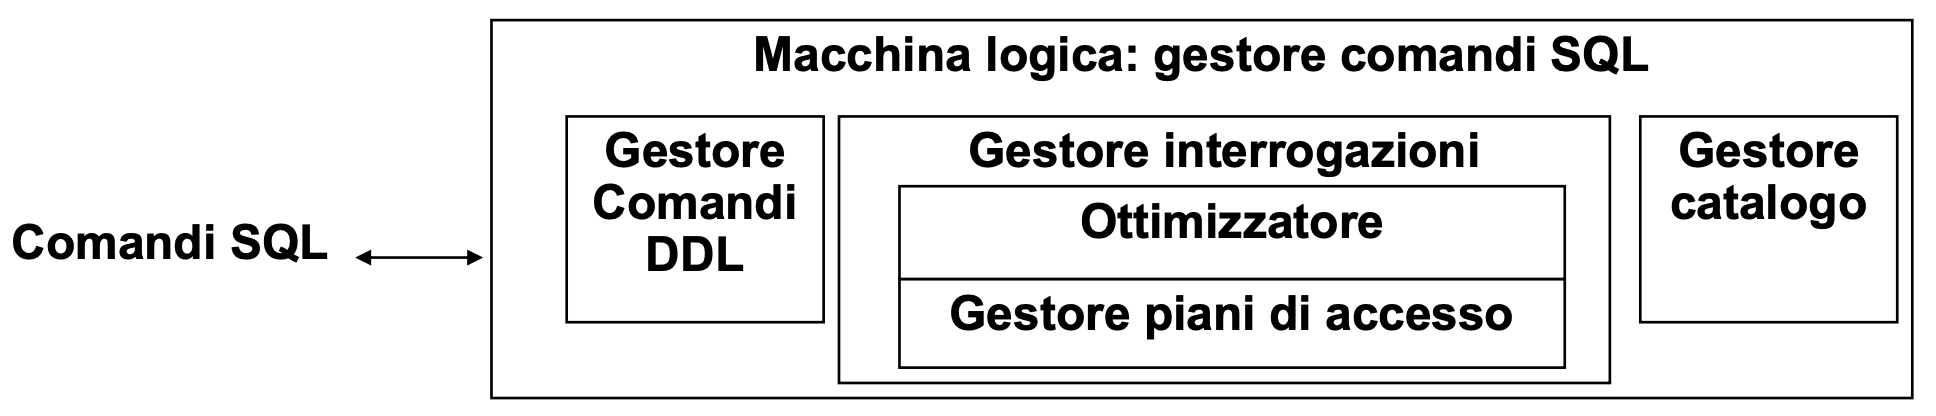
\includegraphics[scale=0.35]{img/piani_accesso.png}
\end{figure}

L'\emph{ottimizzatore} sceglie, in base al comando \emph{SQL}, il piano d'accesso
dal costo minimo, usando le statistiche presenti nel \emph{catalogo}. Nel processo di ottimizzazione,
dati il comando \emph{SQL} e il catalogo, viene prima effettuata una procedura di analisi lessicale e semantica, e di
semplificazione del comando, questa fase dà in output un albero di operatori logici dell'algebra relazionale,
sul quale si esegue una trasformazione utilizzando delle regole di equivalenza. Successivamente si applica
un'ottimizzazione fisica dove gli operatori logici sono trasformati in operatori
fisici e la loro scelta definisce il piano d'accesso. In quest'albero, le foglie sono le tabelle
e i nodi interni specificano le modalità con cui gli accessi e le operazioni relazionali sono effettuate.

\begin{definition}[Piano d'Accesso]
    Scelta dell'algoritmo per eseguire ogni operatore.
\end{definition}

Infatti ogni operatore logico può essere realizzato mediante più algoritmi
che rappresentano gli operatori fisici.

Ogni operatore fisico è un'\textcolor{purple}{\emph{iteratore}}, ovvero un oggetto con i seguenti metodi (realizzati dalla macchina fisica):
\begin{itemize}
    \item \verb|open()|: inizializza lo stato dell'operatore allocando i buffer per gli input e gli output,
        inoltre richiama ricorsivamente la \verb|open()| sugli operatori figli e passa anche i parametri.
    \item \verb|next()|: ritorna la prossima tupla del risultato, include anche la \verb|next()| sui figli.
    \item \verb|isDone()|: indica se ci sono ancora tuple da leggere.
    \item \verb|reset()|.
    \item \verb|close()|: termina l'esecuzione dell'operatore e rilascia le risorse ad esso allocate.
\end{itemize}

Ecco una lista di operatori logici ed i corrispondenti fisici:
\begin{itemize}
    \item \textbf{\textcolor{purple}{R}}:
        \begin{itemize}
            \item \textcolor{purple}{TableScan(R)}: per la scansione della relazione $R$.
            \item \textcolor{purple}{IndexScan(R, Idx)}: scansione di $R$ utilizzando l'indice $Idx$.
            \item \textcolor{purple}{SortScan(R, $\{A_i\}$)}: scansione di $R$ ordinata sull'insieme $\{A_i\}$.
        \end{itemize}
    \item \textbf{\textcolor{purple}{$\pi_{A_i}$}}:
        \begin{itemize}
            \item \textcolor{purple}{Project(O, $\{A_i\}$)}: per la proiezione dei record di $O$ senza eliminare i duplicati.
            \item \textcolor{purple}{Distinct(O)}: per eliminare i duplicati dei record ordinati di $O$.
        \end{itemize}
    \item \textbf{\textcolor{purple}{$\sigma_{\Psi}$}}:
        \begin{itemize}
            \item \textcolor{purple}{Filter(O, $\Psi$)}: per la restrizione dei record di $O$ senza indici.
            \item \textcolor{purple}{IndexFilter(R, Idx, $\Psi$)}: per la restrizione con indice dei record di $R$.
                Ovviamente, gli attributi utilizzati nella condizione $\Psi$ devono essere gli stessi presenti nell'indice $Idx$.
        \end{itemize}
    \item \textbf{\textcolor{purple}{$\tau{\{A_i\}}$}}:
        \begin{itemize}
            \item \textcolor{purple}{Sort(O, $\{A_i\}$)}: per ordinare i record di $O$ per valori crescenti degli $\{A_i\}$.
        \end{itemize}
    \item \textbf{\textcolor{purple}{$\{A_i\}\gamma\{f_i\}$}}:
        \begin{itemize}
            \item \textcolor{purple}{GroupBy(O, $\{A_i\}$, $\{f_i\}$)}: per raggruppare i record di $O$ sugli attributi
                $\{A_i\}$ e usando le funzioni di aggregazione in $\{f_i\}$. In $\{f_i\}$ vi sono le funzioni presenti
                nella \verb|SELECT| e nella \verb|HAVING|. I record di $O$ devono essere ordinati sugli $\{A_i\}$.
        \end{itemize}
    \item \textbf{\textcolor{purple}{$\bowtie_{\Psi_J}$}}:
        \begin{itemize}
            \item \textcolor{purple}{NestedLoop($O_E, O_I, \Psi_J$)}: in questo caso, semplicemente,
                il \emph{NestedLoop} invoca la \verb|next()| prima su $O_E$ e poi su $O_I$, poi esegue
                la condizione e se è rispettata aggiunge la nuova tupla al risultato, in seguito ripete questa
                procedura iterativamente con le \verb|next()| finchè non ci sono più tuple di $O_E$ e $O_I$.
            \item \textcolor{purple}{PageNestedLoop($O_E, O_I, \Psi_J$)}.
            \item \textcolor{purple}{IndexNestedLoop($O_E, O_I, \Psi_J$)}: L'operando interno ($O_I$), deve essere un \emph{IndexFilter($R$, $Idx$, $\Psi^{'}_J$)}
                oppure dev'essere un \emph{Filter($O$, $\Psi^{''}$)} dove $O$ è comunque
                un \emph{IndexFilter($R$, $Idx$, $\Psi^{'}_J$)}. La condizione $\Psi^{'}_J$ è uguale
                alla condizione di giunzione $\Psi_J$, solo che a runtime gli attributi di $O_E$ sono sostituiti
                dai valori presenti per ogni tupla $r$ di $O_E$.
                
                A livello procedurale, qui è un po' diverso rispetto al \emph{Nested Loop}. La \emph{IndexNestedLoop},
                invoca prima la \verb|open()| su $O_E$ e per ogni tupla restituita dalla \verb|next()|,
                utilizza la \verb|open()| su $O_I$ passandogli come parametri i valori degli attributi di $O_E$ presenti
                nella condizione di \verb|JOIN|, cosicchè l'\emph{IndexFilter} presente in uno dei livelli inferiori
                possa restituire le tuple che rispettano la condizione (che come detto prima cambia a runtime); successivamente
                l'\emph{IndexNestedLoop} chiamarà iterativamente la \verb|next()| su $O_I$ per ottenere queste tuple.
            \item \textcolor{purple}{SortMerge($O_E, O_I, \Psi_J$)}.
        \end{itemize}
\end{itemize}

È importante sottolineare che gli operatori che presentano $R$ sono quelli
che operano direttamente sulle tabelle, e che quindi nell'albero sono sempre delle
foglie, mentre gli operatori che presentano $O$ operano su un oggetto che è il risultato
di un altro nodo nel livello inferiore.